\section{Experiments}

\subsection{Monk's results}
\begin{table}[H]
\begin{tabular}{|c|c|c|c|c|c|c|}
\hline
\textbf{Task} &	\textbf{\#Units} &\textbf{ eta} & \textbf{lambda} &\textbf{momentum} & {\textbf{MSE(TR/TS)}} &\textbf{Accuracy(TR/TS)} \\ \hline
MONK 1        &    3 & 0.9 & 0 & 0.7  &   6.2e-4/1e-3 &   100\%/100\%  \\ \hline
MONK 2        &    4 & 0.8 & 0 & 0.7  &   5.2e-3/6.9e-3 &   100\%/100\% \\ \hline               
MONK 3        &    5 & 0.4 &1e-3 &0.2&     4.1e-2/2.5e-2&    93.44\%/97.22\%  \\ \hline
MONK 3 (no reg)&   5 & 0.8 &   0 &  0.7 &   1.8e-2/2.6e-2 & 95.90\%/\%93.51		\\ \hline              
\end{tabular}
\end{table}
\subsubsection{Monk 1}
\begin{figure}[H]
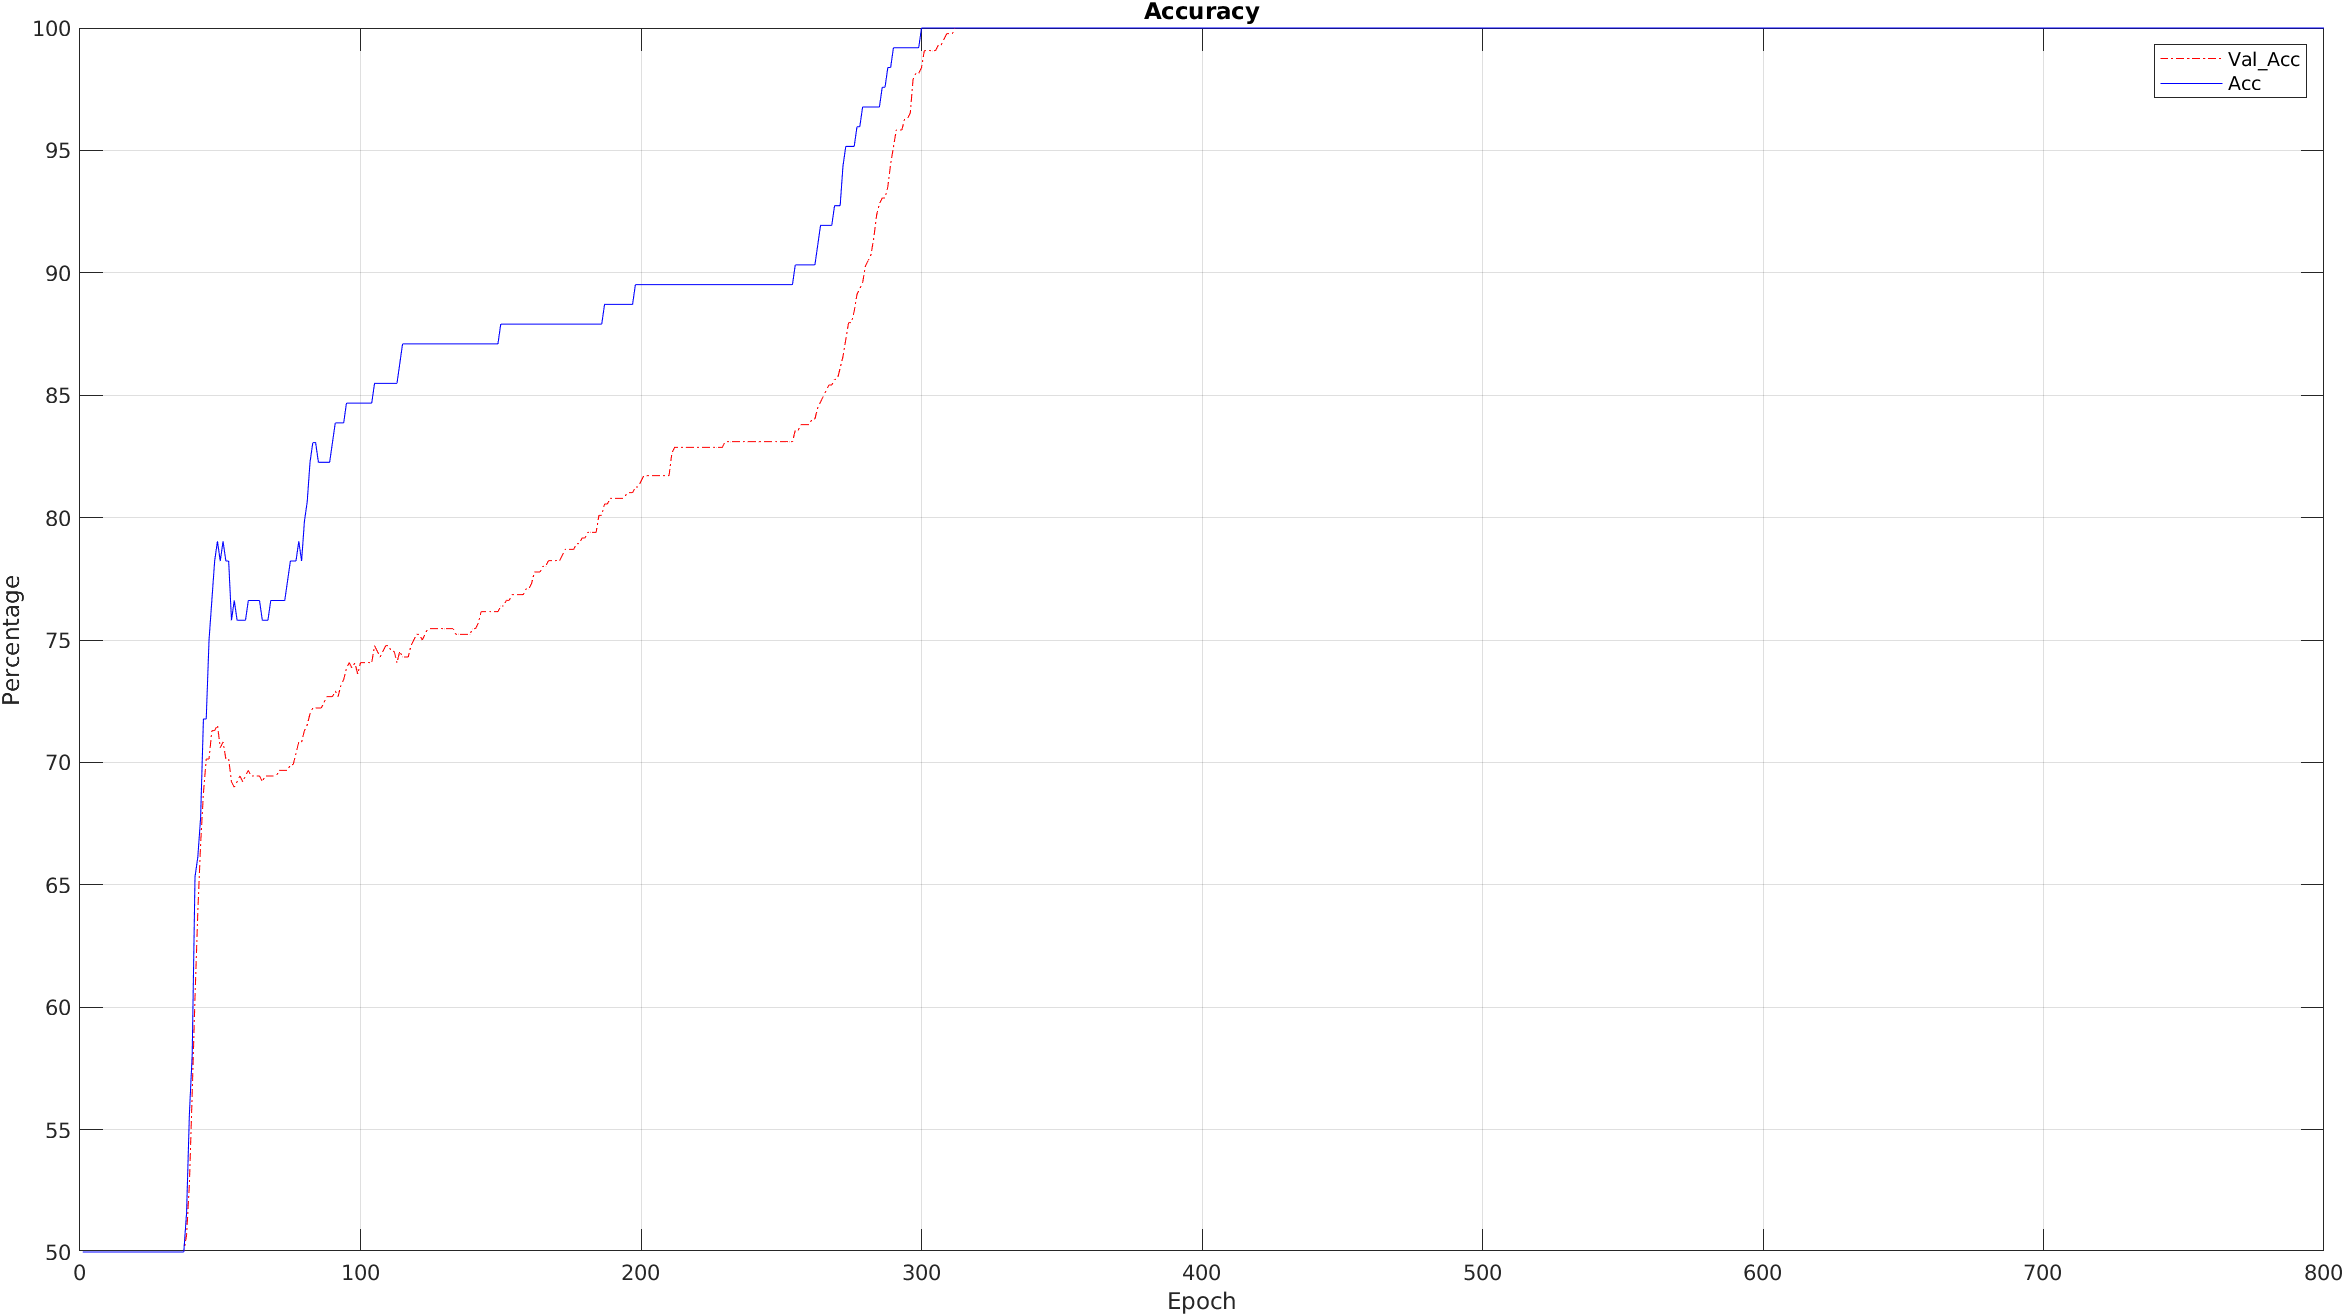
\includegraphics[scale=0.2]{img/Monk1_accuracy.png}
\caption{Accuracy Monk 1}
\end{figure}

\begin{figure}[H]
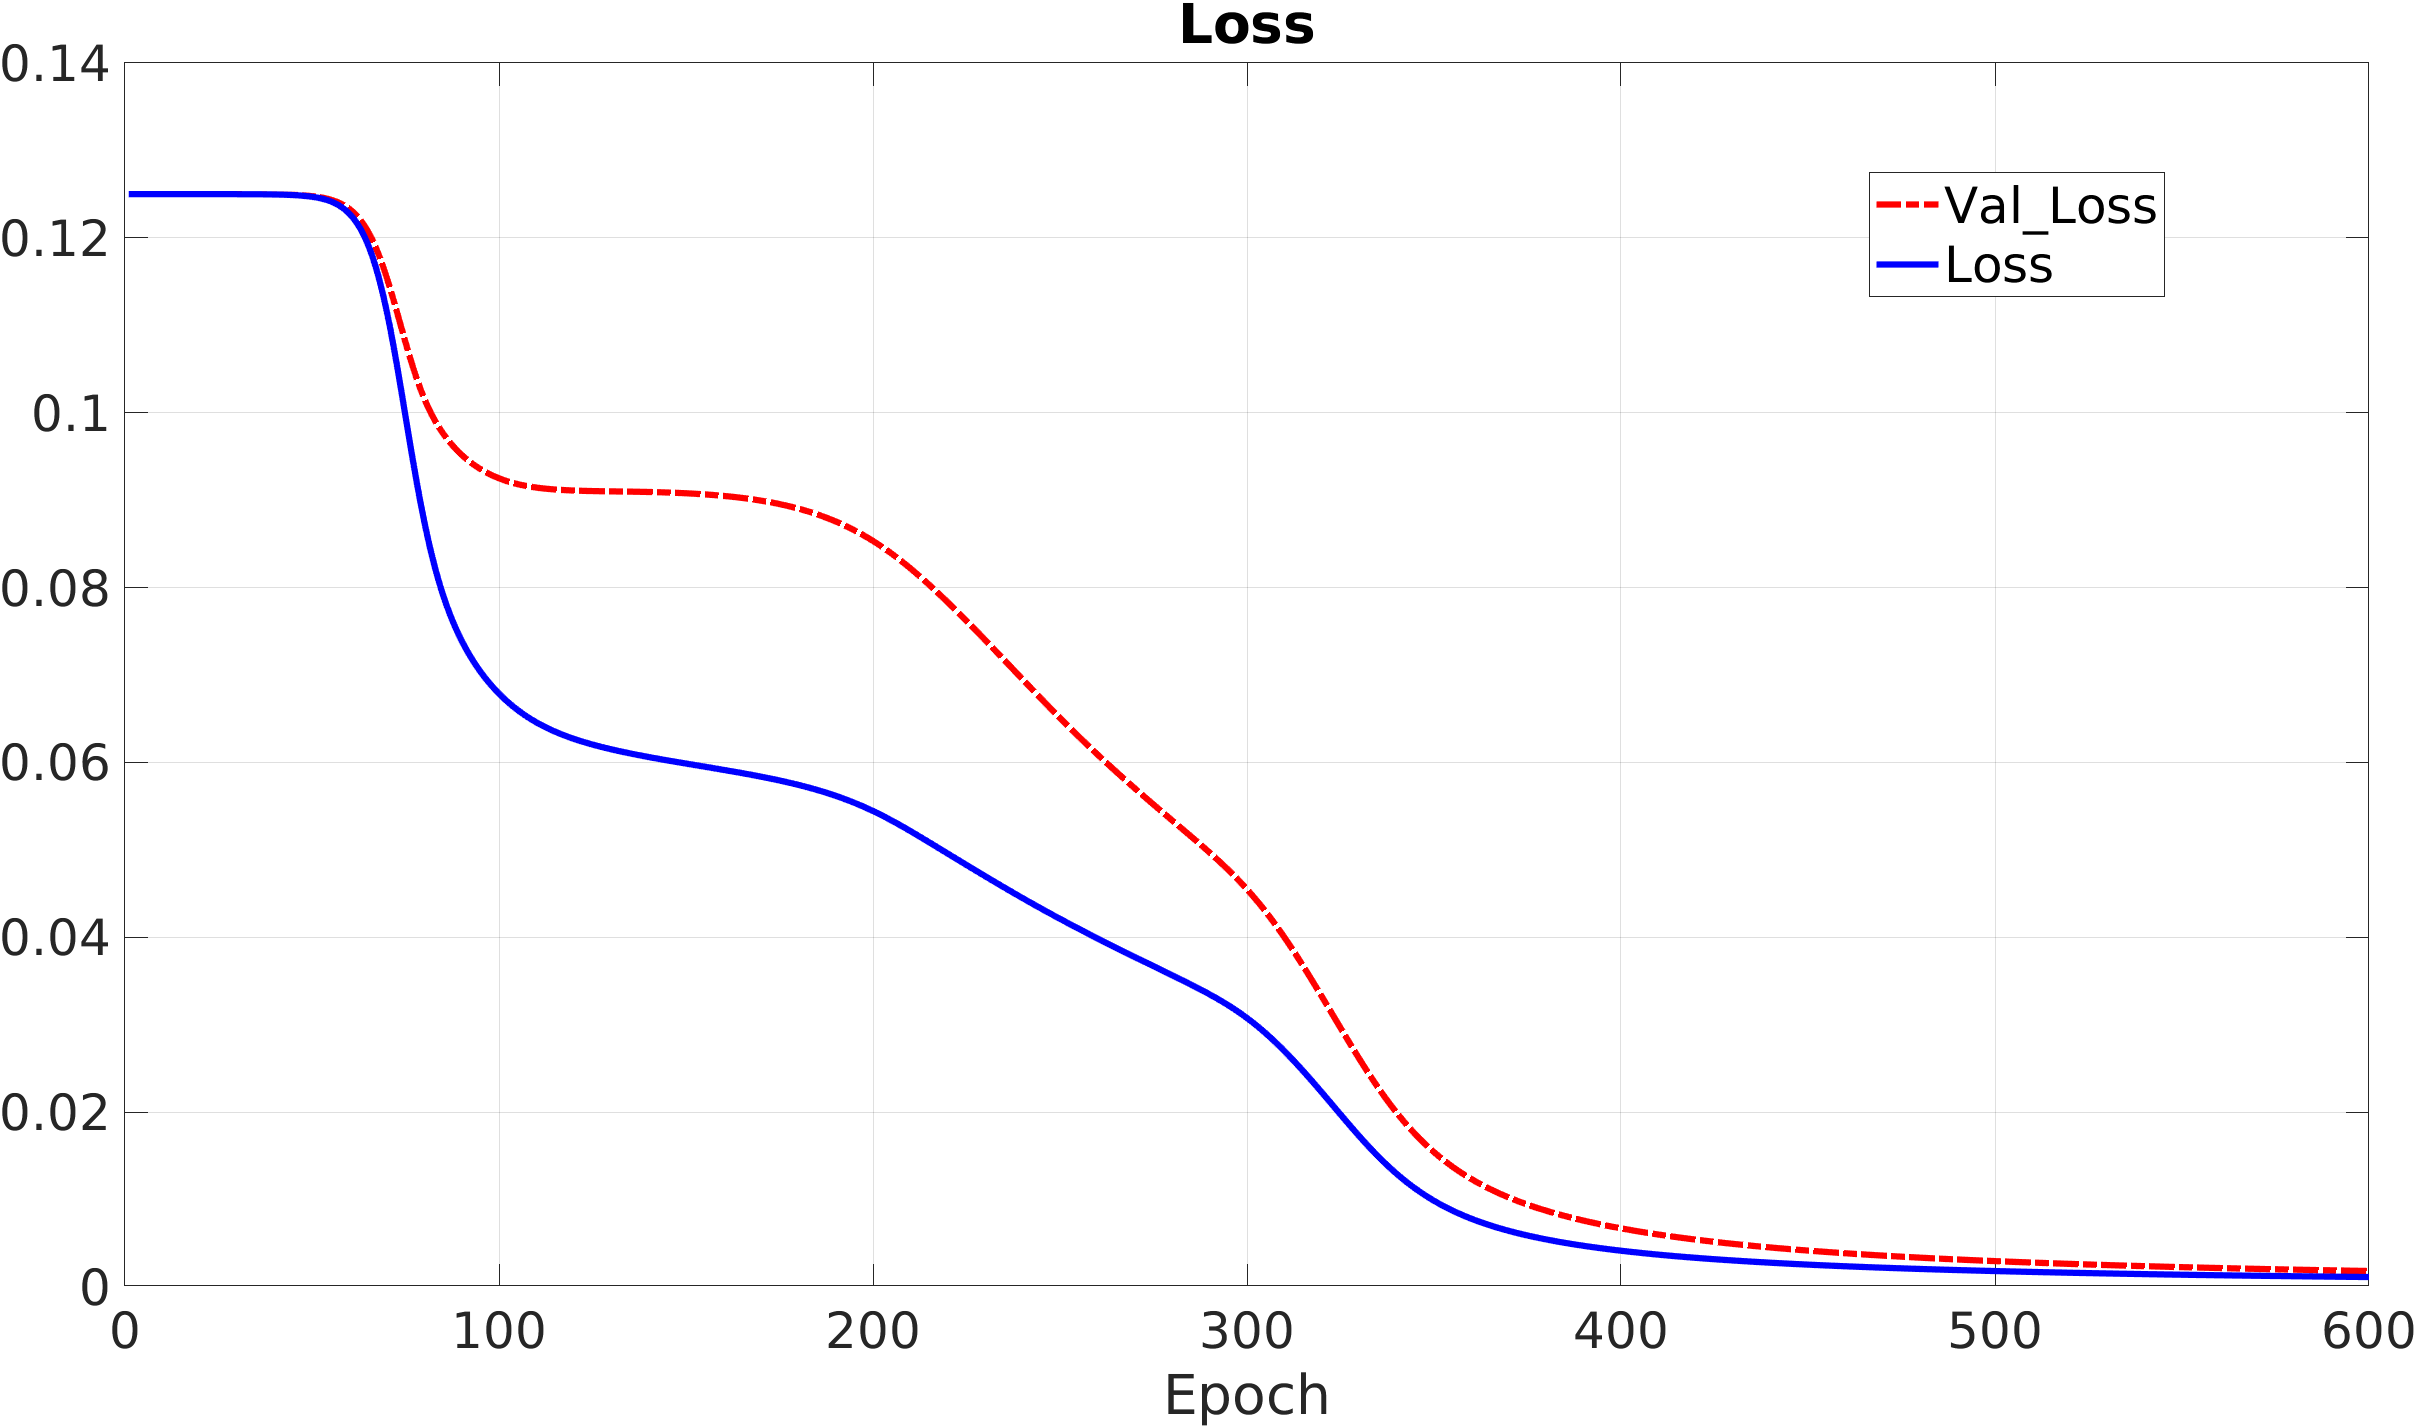
\includegraphics[scale=0.2]{img/Monk1_loss.png}
\caption{MSE curve Monk 1}
\end{figure}


\subsubsection{Monk 2}
\begin{figure}[H]
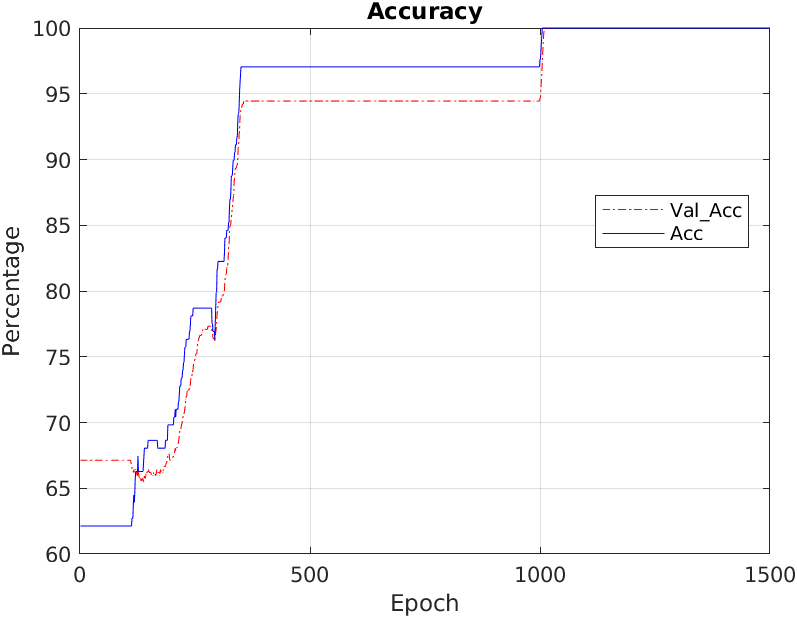
\includegraphics[scale=0.2]{img/Monk2_accuracy.png}
\caption{Accuracy Monk 2}
\end{figure}

\begin{figure}[H]
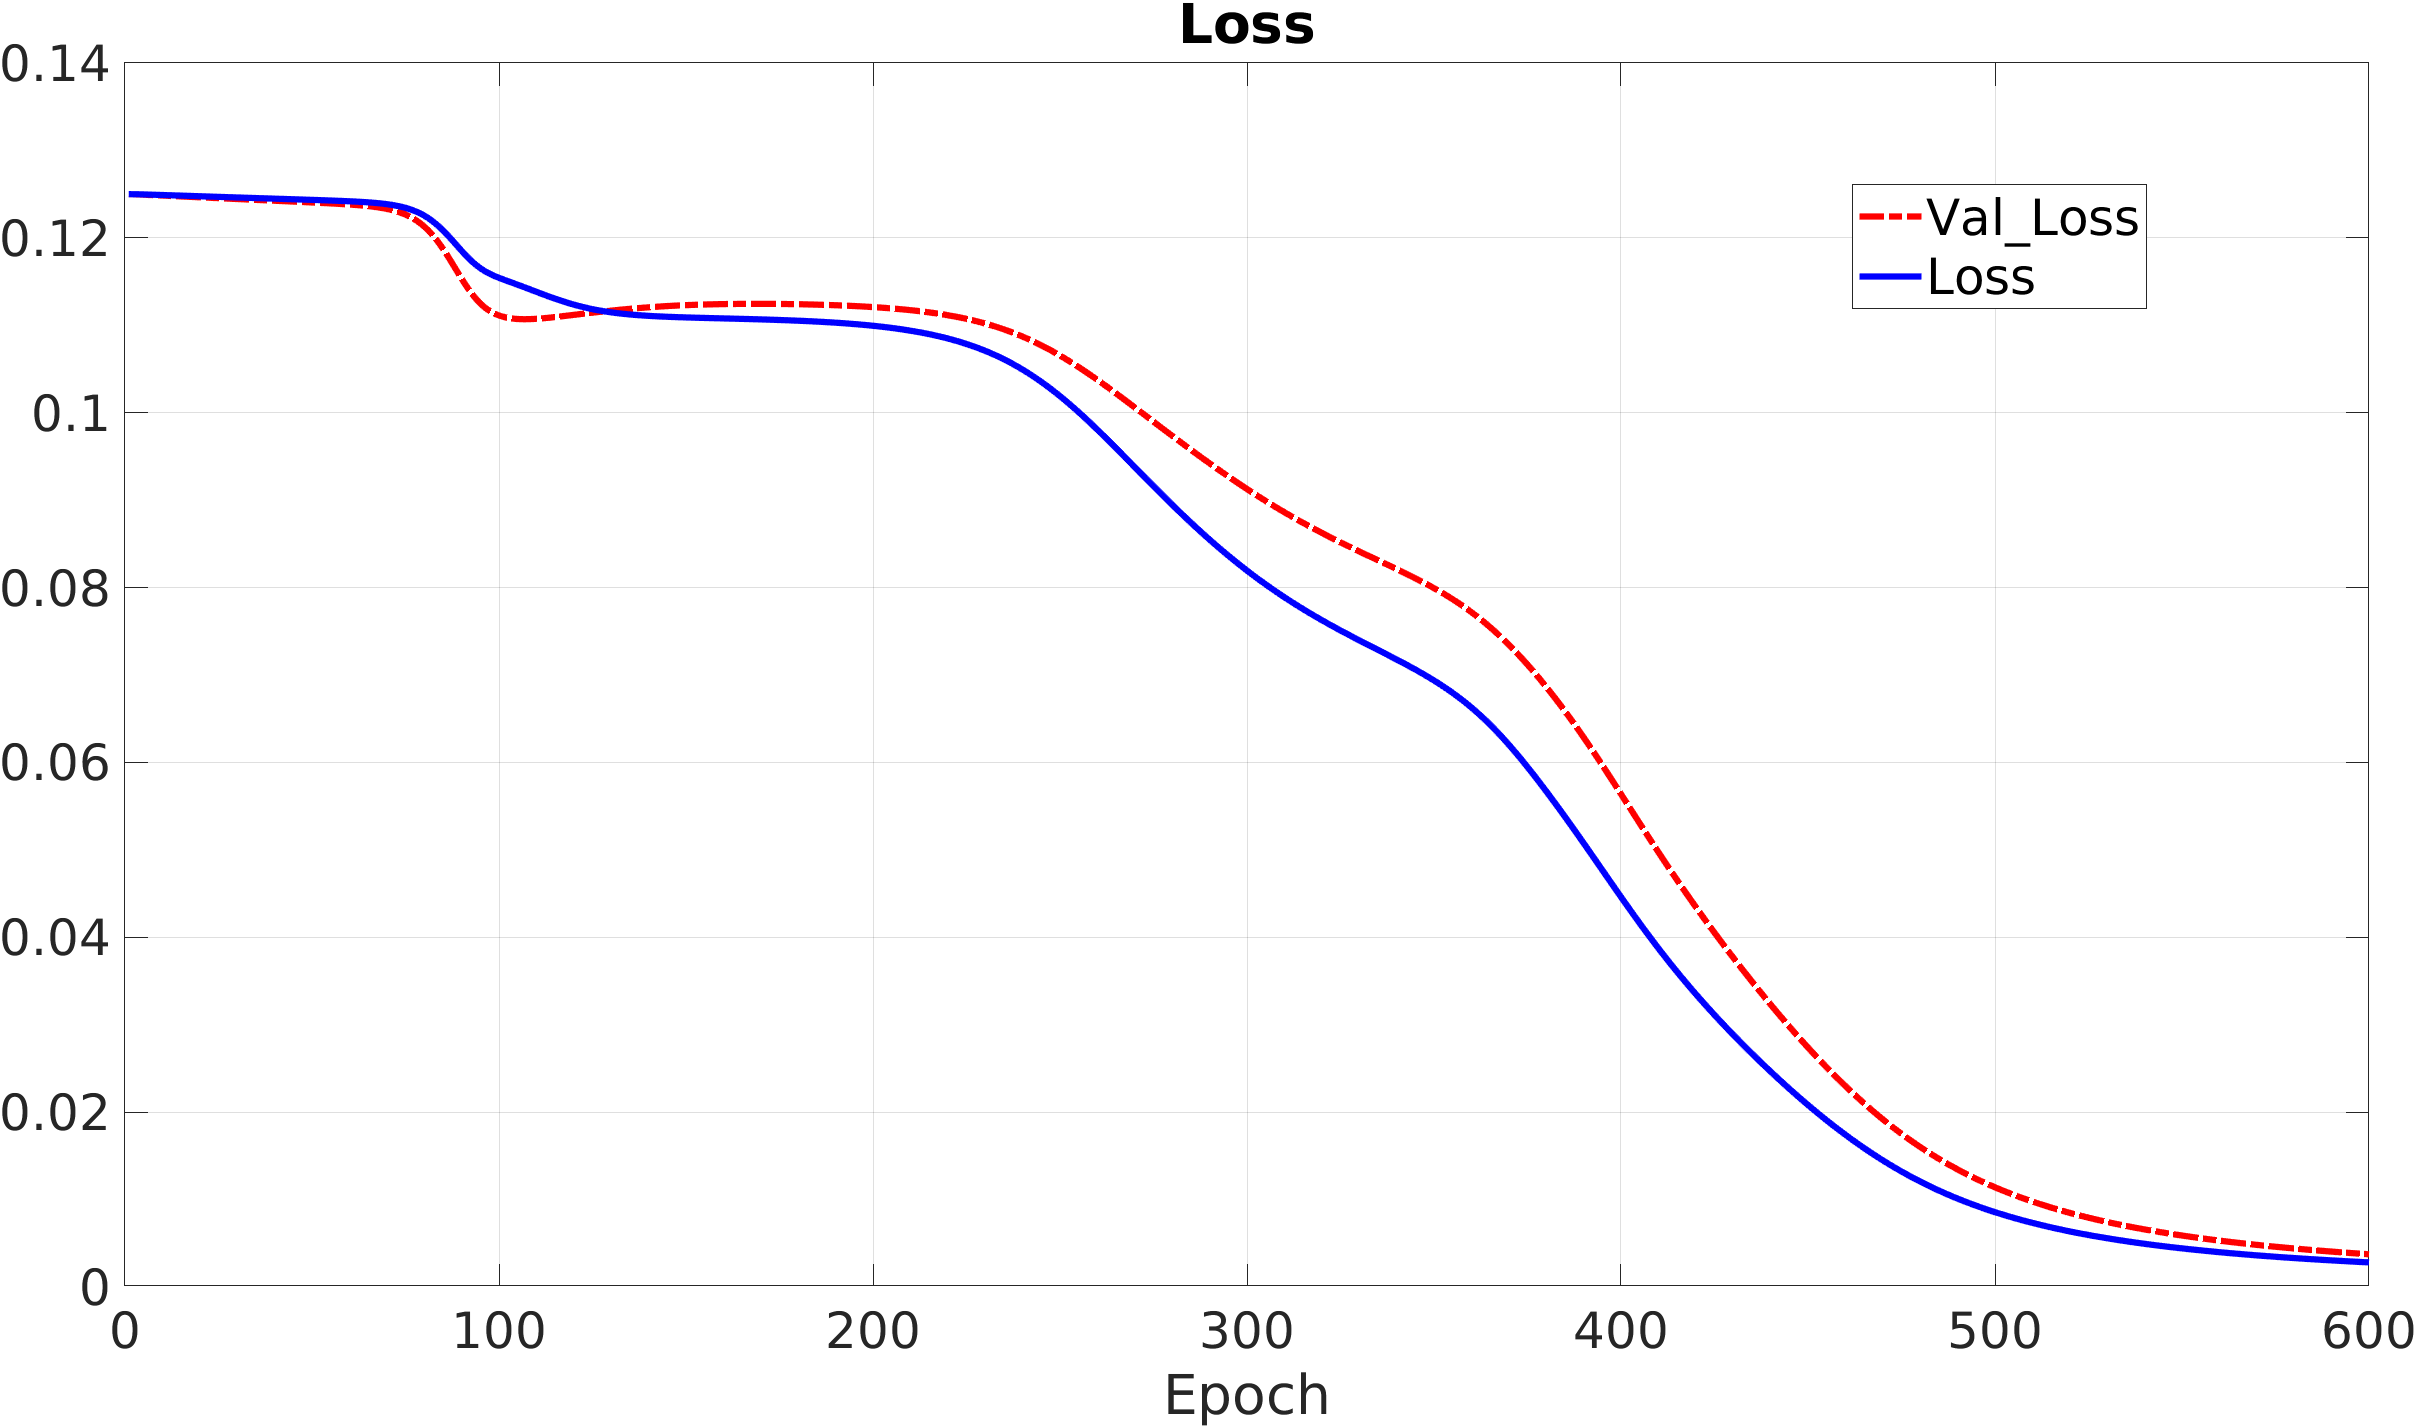
\includegraphics[scale=0.2]{img/Monk2_loss.png}
\caption{MSE curve Monk 2}
\end{figure}

\subsubsection{Monk 3}

\begin{figure}[H]
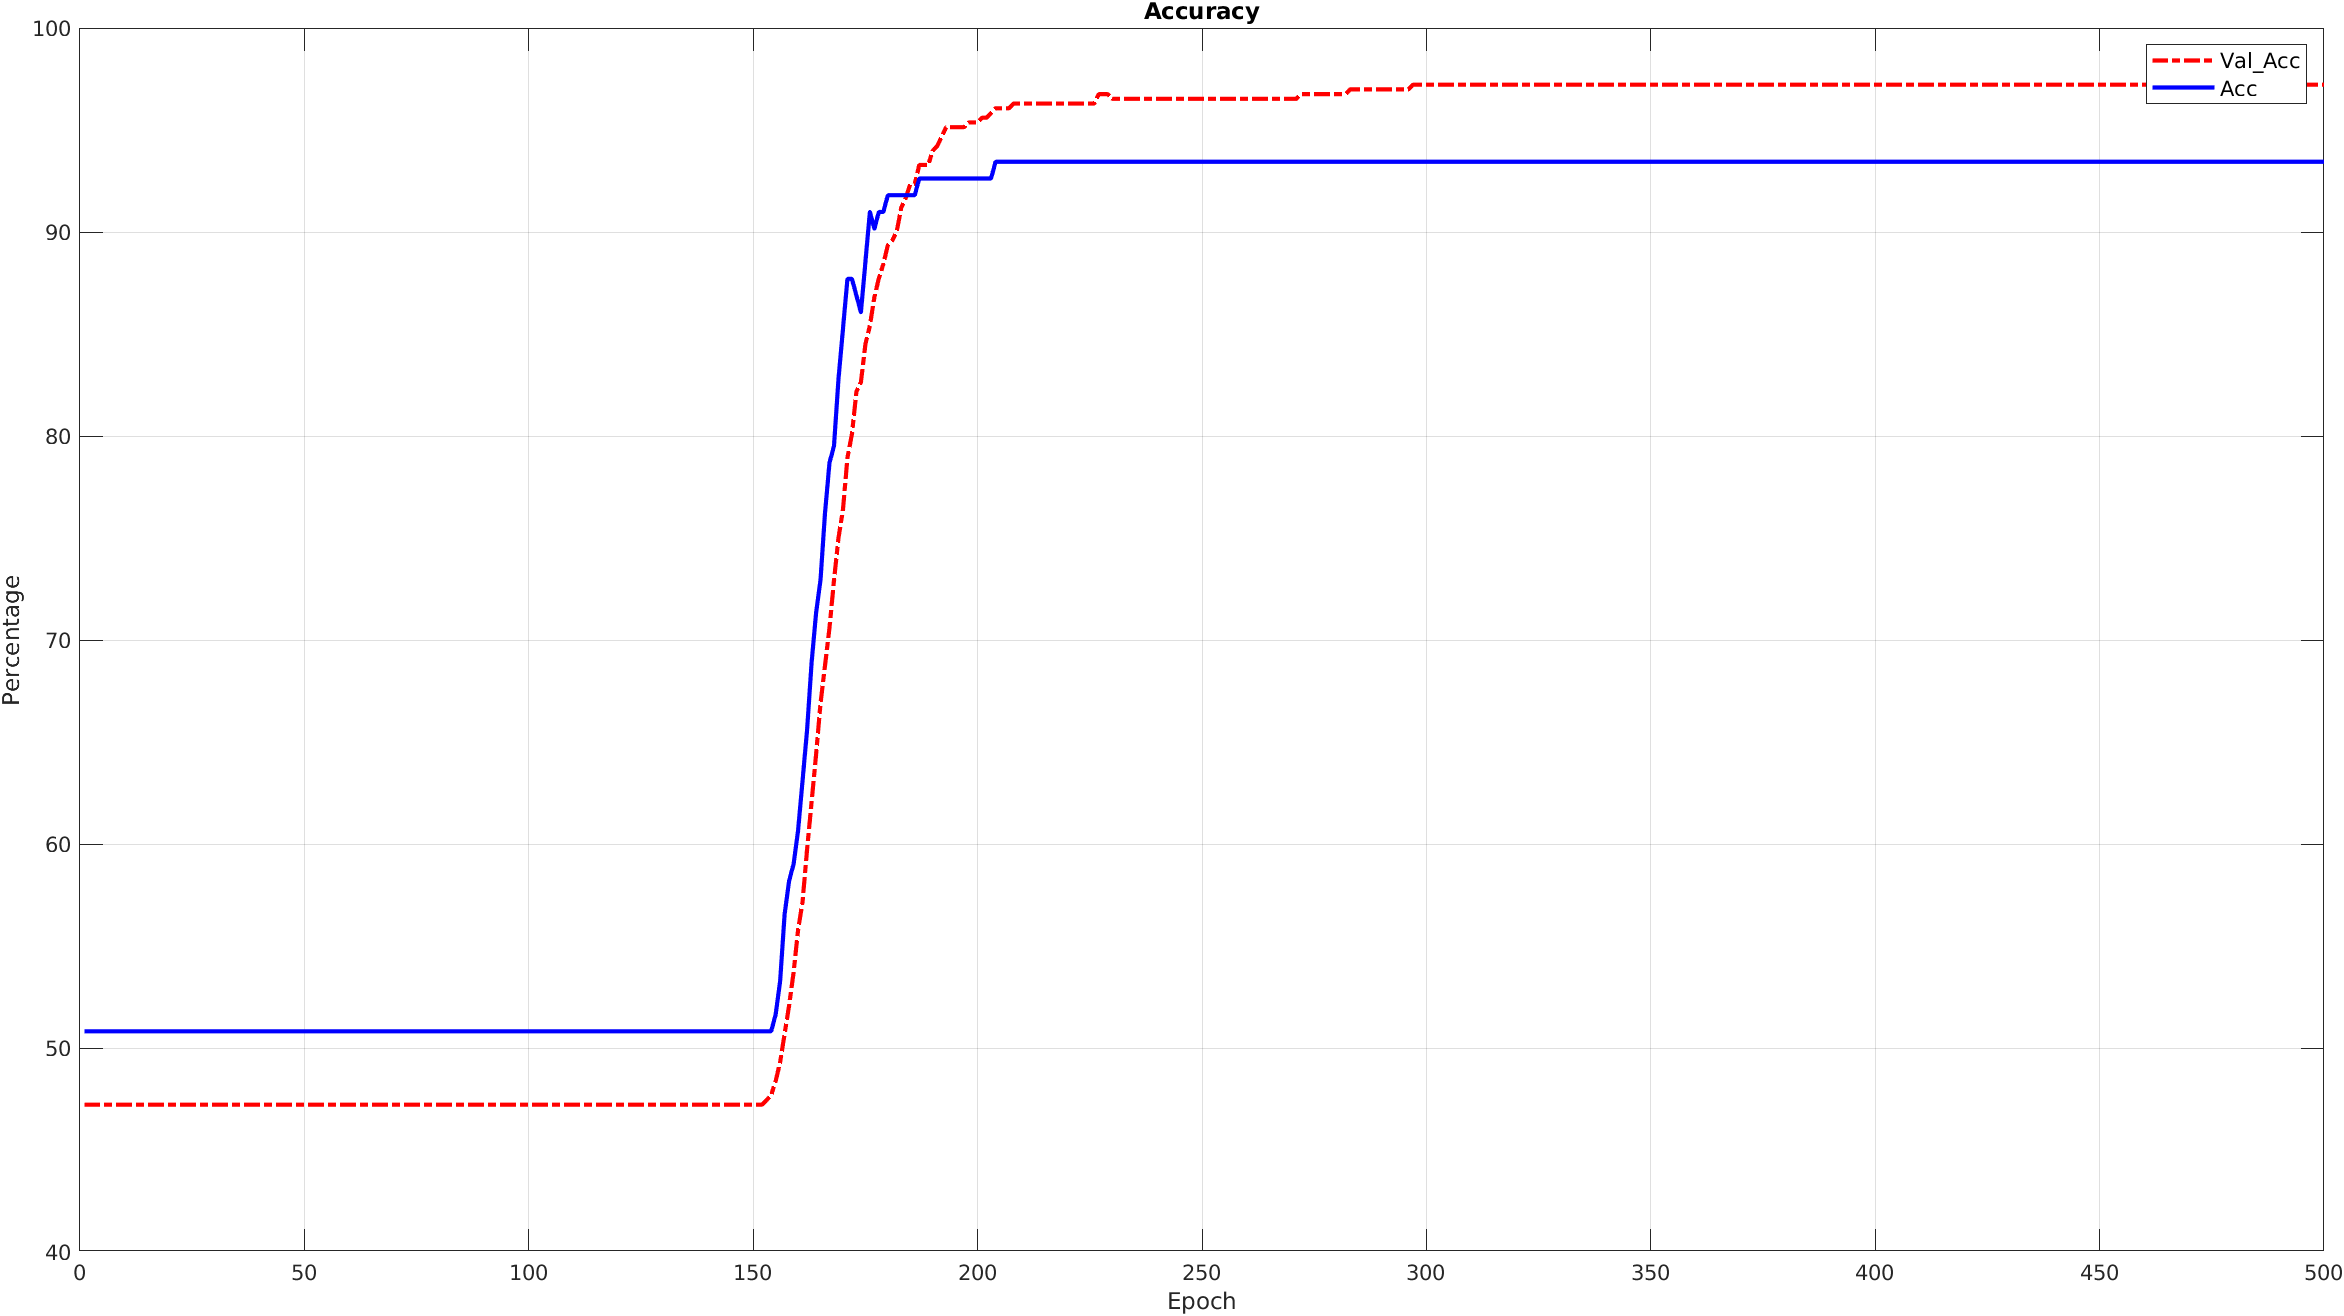
\includegraphics[scale=0.2]{img/Monk3_accuracy_Reg.png}
\caption{}
\end{figure}

\begin{figure}[H]
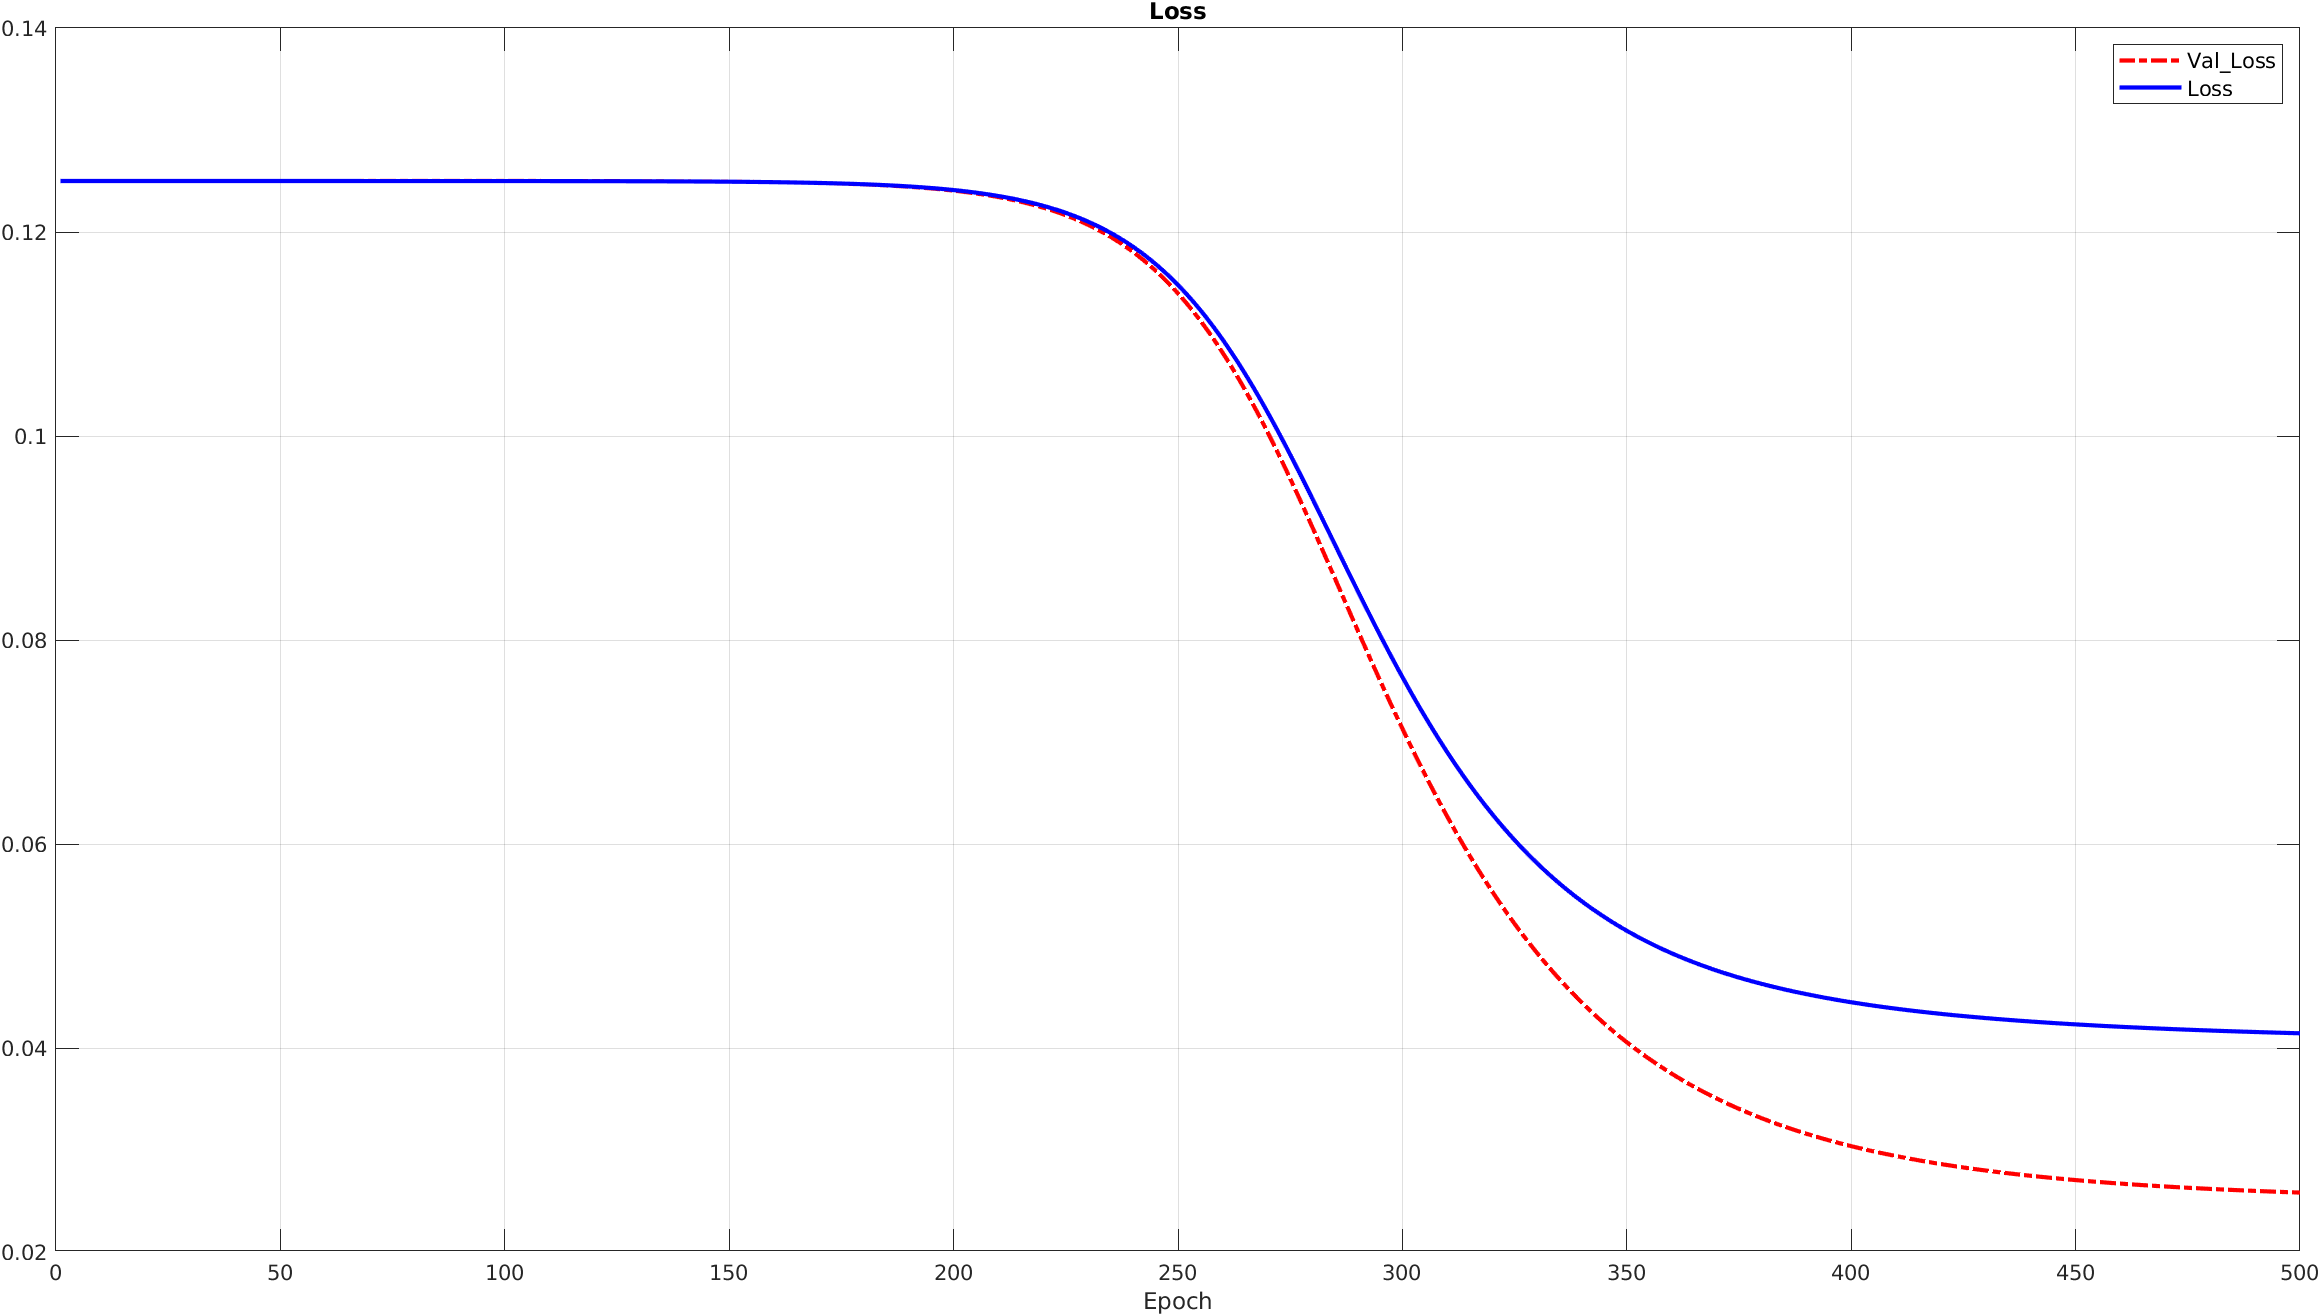
\includegraphics[scale=0.2]{img/Monk3_loss_Reg.png}
\caption{}
\end{figure}

\subsection{Cup results}